\documentclass{article} % For LaTeX2e
\usepackage{nips13submit_e,times}
\usepackage{hyperref}
\usepackage{url}
\usepackage{graphicx} 
\usepackage[caption=false,font=footnotesize]{subfig}
\usepackage{amsmath}
\usepackage{amssymb}
\renewcommand{\figurename}{\bf Figure}
%\documentstyle[nips13submit_09,times,art10]{article} % For LaTeX 2.09


\title{Biometric in Motion: Identification Using Acceleration Data}


\author{
Zexi Mao\\
\texttt{zexim@andrew.cmu.edu} \\
\And
Siqi Tan \\
\texttt{siqitan@andrew.cmu.edu} \\
\AND
Yuchen Wu\\
\texttt{yuchenw@cs.cmu.edu} \\
\And
Yimeng Zhang \\
\texttt{yimengzh@cmu.edu} \\
}

% The \author macro works with any number of authors. There are two commands
% used to separate the names and addresses of multiple authors: \And and \AND.
%
% Using \And between authors leaves it to \LaTeX{} to determine where to break
% the lines. Using \AND forces a linebreak at that point. So, if \LaTeX{}
% puts 3 of 4 authors names on the first line, and the last on the second
% line, try using \AND instead of \And before the third author name.

\newcommand{\fix}{\marginpar{FIX}}
\newcommand{\new}{\marginpar{NEW}}

\nipsfinalcopy % Uncomment for camera-ready version

\begin{document}


\maketitle

\begin{abstract}
As cellphones and other smart devices are closer to our daily life than ever, we are curious to know how the data gathered by accelerometers on them impact our lives, particularly in terms of identifying users of devices via such data. In this project, we try to answer this question with machine learning techniques. We first studied how to implement such biometric techniques by retrieving useful identification information from raw accelerometer data. We then built classifiers with these information. At last we investigated in what way and how much of our privacy leaks through this technique via cellphones. We hope this work could show how such techniques impact our lives.
\end{abstract}

\section{Introduction}

\subsection{Motivation}

\emph{Why is it important} Ubiquitous computing had never been so close to us as our phones become smarter and more powerful today. Sensors equipped in our cellphones like GPS, gyroscope, accelerometer and even barometer collect data from the surrounding environment and ourselves. This information collected from our cellphones and other mobile devices can boost many more applications than just adjusting the brightness of the screen and rotating it automatically. Google uses the GPS data from our phones to provide real-time traffic conditions. Apps can track how well you sleep by just putting your phone beside you on bed. Indoor localization takes advantage of wireless fingerprint, sound from microphone, footsteps from accelerometer and even colors from the camera to tell you where you are when GPS signal is weak inside buildings. Fancier applications far beyond the original purposes of these sensors are on the way. How to retrieve more information from the raw sensor data is one of the hottest and promising topics today.

\emph{What is the problem} Accelerometer is one of the most interesting sensors in our cellphone, which records the acceleration data in 3D. Posture of the phone, gestures and footsteps of the user, and even the user's sleeping condition can be measured by the accelerometer.

In this project, we tried to explore a novel usage of the accelerometer: biometric identification. In other words, can we identify the user by only looking into how he (she) moves? We believe that everyone has his (her) own unique pattern of movement. If this assumption is true, we can identify the person when we match the current data from the accelerometer with the historical data we have learned. 

\emph{Brief outline of solution} In this project, we chose the already available accelerometer dataset gathered by Kaggle. Due to the poor quality of the raw data set, we first performed preprocessing. The goal of preprocessing is to normalize data for easier feature extraction. Then we extracted discriminative features from the preprocessed dataset. The features we used included frequent domain patterns, relative and absolute time domain relations. We applied several classifiers to the feature vectors. So far, we have got a score of over 0.90 in terms of area under the ROC curve, which is satisfactory, although further improvement is still needed.

Furthermore, we studied how the features we used impacts the accuracy of identification. We also showed the relation between quantity of training data and accuracy. These results help us understand what leaks our private information and how to stop it.






\subsection{Related Work} 

A human being's walking gait can reflect the walker's physical characteristics and psychological state, and therefore the features of gait can be employed for individual recognition. The use of accelerometer data for biometric identification is relatively new but has been increasingly explored in recent years. Existing methods for gait recognition have shown good performance.
 
Gafurov et al. \cite{Gafurov:AIAT2007} attach multiple sensors to a subject at different body parts. Xu et al. \cite{Xu:ICB2012} developed an Android App to collect gait acceleration data. With a reasonably sized dataset, by matching gait patterns across different paces, they show preliminary results indicating that not only can smart phones be used to identify a person based on their normal gait but also that there is potential to match gait patterns across different speeds.

Tao et al.\cite{Tao:ToPAMI2007} focus on the representation and pre-processing of appearance-based models for human gait sequences. Two major novel representation models are presented, namely, Gabor gait and tensor gait. Experiments show that the new algorithms achieve better recognition rates than previous algorithms.

Pan et al. \cite{Pan:EL2009} proposed algorithm based on signature points, instead of the whole gait signal. They consider acceleration-based gait recognition insensitive to changes of lighting conditions and viewpoint. Their algorithm firstly extracts signature points from gait acceleration signals, and then identifies the gait pattern using a signature point-based voting scheme. The experimental results shows the accelerometer-based gait biometrics is promising. 

Kwapisz et al.\cite{Kwapisz:BTAS2009} collect some data and also perform identification experiments . Based on the 600 raw accelerometer readings, they generated 43 features, which are variations of 6 basic features including average acceleration value, standard deviation, time between peaks and so on. They applied two classification techniques decision trees neural networks to classify and the identification performance turned out to be fairly good.


\section{Information on the Kaggle competition}
\subsection{Raw data}
The dataset provided by the Kaggle competition \href{http://www.kaggle.com/c/accelerometer-biometric-competition}{``Accelerometer Biometric Competition''}. The dataset consisted of 3 parts: a training set, a testing set and a question set. Each single sample point in training and testing sets contained a time stamp in milliseconds, acceleration measurements in 3 dimensions, and an associated DeviceId (for the training set) or a SequenceId (for the testing set). 

In the training set, there were 30 million samples, which were collected from 387 different devices as labeled. These samples were demarcated into 387 segments, each containing samples for a single device. In the testing data set, there were also about 30 million samples without label. These samples were demarcated into 90,024 sequences of 300 points, each with a SequenceId. In the question set, for each SequenceId, there was a proposed DeviceId.

\subsection{Evaluation}
The task on Kaggle was to tell whether each sequence's proposed DeviceId was the sequence's real DeviceId. For each sequence, we were required to give a belief, in real number, about the credibility of the proposed DeviceId. This competition was designed to investigate the feasibility of using accelerometer data as a biometric for identifying users of mobile devices. For more detail, please refer to the competition website as listed above.

We should emphasize our goal of this project is not simply performing well in the Kaggle competition, but aims at how such technique impacts our daily life. However, for fairly evaluating our approach, we use the Kaggle online judging system along with hundreds of other teams. This system automatically outputs the area under the ROC curve as the score for a submitted answer generated by our classifiers. 


\section{Methods}
In this section, we describe the methods we have used for preprocessing, feature extraction, and classification. This is not necessarily the final version of our approach. 


\subsection{Preprocessing}
There were two problems with the raw dataset for further processing: 1) accelerometer data for each device was not properly segmented; 2) accelerometer readings were not uniformly sampled. For the first problem, we performed segmentation on both training sequences and testing sequences. For the second problem, we performed re-sampling based on cubic spline interpolation.

\begin{figure}
    \hspace{-0.5cm}
    \begin{minipage}[t]{0.02\textwidth}~
    \end{minipage}
    \begin{minipage}[t]{0.47\textwidth}
    \centering
    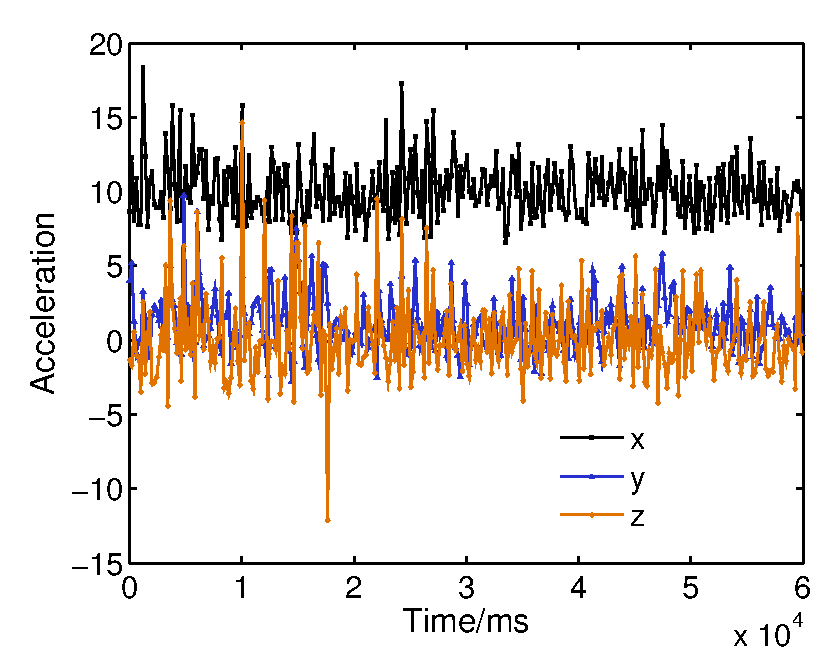
\includegraphics[height=40mm]{fig/good_raw.eps}
    \caption{A good sequence from raw data. Samples points were close in time. We regarded these points as representing a single activity.}
    \label{fig:good_raw}
    \end{minipage}
    \begin{minipage}[t]{0.02\textwidth}~
    \end{minipage}
    \begin{minipage}[t]{0.47\textwidth}
    \centering
    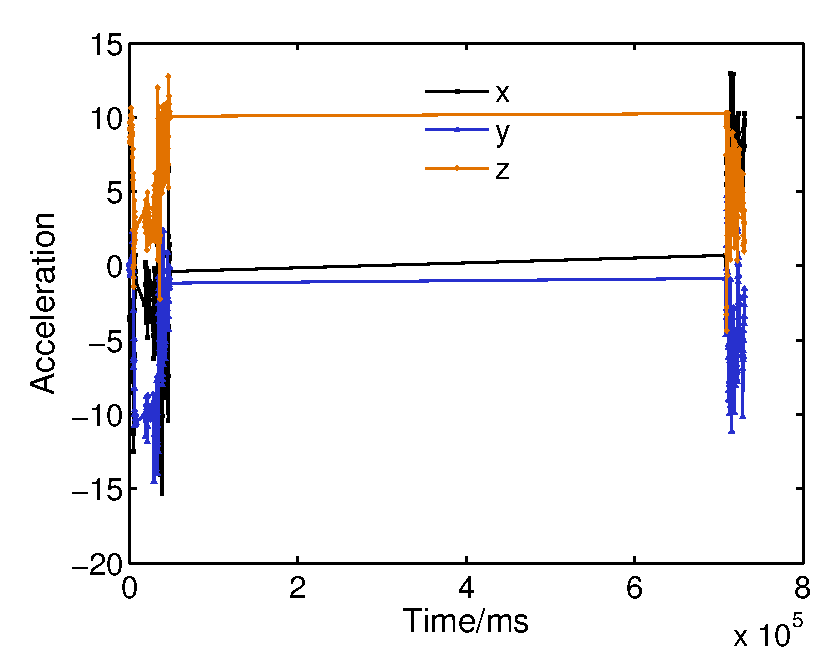
\includegraphics[height=40mm]{fig/bad_raw.eps}\\
    \caption{A bad sequence from raw data. This piece essentially contains information about 2 separate activities that were far apart in time. The line segments in the middle of the figure was due to the large time intervals between adjacent sample points.}
    \label{fig:bad_raw}
    \end{minipage}
    \begin{minipage}[t]{0.02\textwidth}~
    \end{minipage}%   
 \end{figure}


\subsubsection{Segmentation} % (fold)
First, the raw data was not properly segmented. For each sequence, the time intervals between two adjacent sample points were less than 500 ms most of the time. However, some intervals could be as huge as 100,000 ms. This problem was illustrated in Figures \ref{fig:good_raw} and \ref{fig:bad_raw}. They contain two test sequences of 300 points. In the first sequence (Figure~\ref{fig:good_raw}), all the points were close in time, and we could regard these points as representing a single activity. In the second sequence (Figure~\ref{fig:bad_raw}), there were two points that were far apart in time (so all the other points were pushed to two sides of the figure), and we can consider this sequence containing information about two separate activities. 

Clearly, we couldn't consider the second sequence as representing information for a single activities, since so much information was unknown between the two far apart sample points. Such huge time interval was not uncommon in the dataset. %This could be attributed to two reasons: 1) in preparing this dataset, sequences of samples during periods of rest exceeding 10 seconds were removed by Kaggle; 2) the device could be off or the app could be closed during the whole data collection process. 

To overcome this problem, we performed segmentation on the raw data to split each sequence into subsequences. Our segmentation had two phases. In the first phase, we split the sequence at points where the time interval was larger than $T_\mathrm{split}$. After this, for each original sequence, we got several shorter sequences that had sample points close in time. In the second phase, we continually split the longest subsequence among all the subsequences until 1) we got $k_\mathrm{\#seq}$ subsequences, or 2) the longest subsequence was shorter than $2 l_\mathrm{maxL}$. Also, sequences shorter than $T_\mathrm{short}$ were thrown.

We did the second-phase segmentation because after the first-phase segmentation, some resultant sequences were too short (less than 1000 ms) so that not much reliable features could be extracted, and some were too long (longer than 100 seconds) so that it might contain information about multiple activities of the user. 

In this manner, on the one hand, we make more sequences from one device, hopefully keeping more information about the device's diverse patterns. On the other hand, we keep the sequences long enough, so that they contain reliable information about patterns of the device.

\subsubsection{Re-sampling} 
After segmentation, for each device, we got several subsequences. However, these sequences were not uniformly sampled, due to various reasons. To make feature extraction simpler, we interpolated each segment using cubic spline and uniformly re-sampled each sequence with  $\tau_\mathrm{resample}$ being the re-sampling time interval.

\subsection{Feature extraction}
\label{feautures}

After preprocessing, for each raw sequence (from training set or testing set), we got several shorter re-sampled subsequences. In this section, we describe how to extract features sfrom each subsequence.
	
%In the end, for each subsequence, we got a feature vector in $\mathbb{R}^{1290}$. This vector can be decomposed into 3 parts: frequency domain features, time domain features, and accelerometer reading features.
There are six categories of features we investigated. They represent different aspects of patterns from the data.

\subsubsection{Frequency domain features}
We believe the patterns of human mobility is easier to be exploited in frequency domain. To this end, for each subsequence, we first extracted sliding windows of size $w_\mathrm{fft}$ and 50\% overlap (determined empirically). Then we did FFT on all windows. Finally, we calculated the magnitude of all first $(w_\mathrm{fft}/2 + 1)$ coefficients and use the average values over all windows as the frequency domain features for the subsequence. Since there were readings from 3 directions, we have $(w_\mathrm{fft}/2 + 1)\times 3$ values for frequency domain features per subsequence.

\subsubsection{Differences of acceleration}
There could be more patterns and properties if we look beyond frequency domain. One obvious feature is the absolute difference between two adjacent readings of acceleration. This feature indicates how rapidly a person usually handles the phone or moves. It also indicates the environment this person lives. We use the distribution of such differences as the features in this category. Specifically, we compute the histogram of absolute differences between every two adjacent readings for each sequence as the features. 

\subsubsection{Resultant acceleration}
The value of each reading alone could also imply useful information. The resultant acceleration, which is defined as $\sqrt{x^2+y^2+z^2}$, directly evaluates the absolute value of the acceleration the phone suffers from. This value tells us how hard a person usually moves as the force is proportional to the acceleration it measures. The distribution of resultant acceleration is the third feature we used. Like we mentioned above, the histogram of this value is produced for each sequence as one category of its features.

\subsubsection{Components of acceleration}
Inspired by the feature above, separately extracting features among the three dimensions could generate more independent features. For example, a phone could usually lie on the desk which means x axis is more likely to be 10, when another phone's reading for y axis is larger when it is always kept in one's pocket. Three histograms are generated with this theory for every sequences.

These four feature categories are what we mainly focus on. There are also many tricky features which could help us a lot to have a better score in the competition. However, these features could be useless in real world applications. 

\subsubsection{Raw sampling rate}
As the mobile devices people use are increasingly diverse, the characteristics of different devices offer us a set of very distinguishing features for recognizing users. One of these characteristics was the sampling intervals of the devices.

As we observed from the raw data set, sampling intervals of devices has a range of approximately 5-250 ms, and for different devices, the distributions of the sampling intervals were quite different. Thus, for each subsequence, we used the histogram (0-600 ms divided into bins of 20 ms, in total 30 values) of the sampling intervals of the original sequence it came from as the time domain features. 

\subsubsection{Sampling granularity}
Apart from the sampling intervals of devices, we found another set of features with potential ability of distinguishing devices, which was the accelerometer readings.

By observing the data, we found that each kind of device could only provide certain discrete values of accelerometer readings, and this might be due to the limited precision of accelerometers. Thus, the set of accelerometer readings a device can provide is also treated as a set of features. For each subsequence, we used the overlap between the the set of readings from the original sequence it came from and the set of readings from the $i$th device, $i=1,\ldots,387$. Since we had reading from 3 directions, $3\times 387 = 1161$ values constituted the accelerometer reading features for each subsequence.

The two tricky features introduced above help teams with satisfactory scores in the Kaggle competition. These features extract more features for phones (or the accelerometers on them) but not for persons. They could easily fail in real world when a lot portion of people use the same type of phone such as iphone. These feature also fails when a person use several mobile device or change the phone to a new type. 

\subsection{Classification}

Once the key features are extracted, it will not be hard to use well studied and developed classifiers for good results. The basic idea is to leverage various kinds of classifiers and optimize their parameter for more accurate results.

After preprocessing and feature extraction, for each original sequence, we now had several feature vectors associated with it. These vectors were used for classification. For testing, the average of prediction results of all feature vectors associated with a test sequence was used for submission.

We start from some naive classifiers. The performance of K-Nearest-Neighbor depends on the number of K and the definition of distance function. This classifier gave us a baseline result. Then we moved on to popular classifiers such as support vector machines and logistic regression. We will also investigate the impact of the parameters of these classifiers in the following sections about implementation.


\section{Implementation and Evaluation}
In this section we show how our approach performed. We will justify the selection of parameters for preprocessing. We will also show the impact of quantity of training data and different features on results. We hope this could tell us how to prevent leakage of our identity by controlling how much and what kind of accelerometer data to exploit.

\subsection{Evaluation methods and metrics}
We adopt the online judging system of Kaggle for fairness. It could also demonstrate how our approach performs against other teams all over the world. 

The system takes results generated from our classifier as input. For the results, our classifier needs to produce the belief of each sequence and the tagged device id with it. Then, the system produces value of Area under the ROC curve (AUC) as the score. The baseline of AUC is 0.5 which stands for purely random guesses. As the higher AUC value, the better classifier we have, a result with AUC of value 1 stands for perfect guess. 

\subsection{Parameter selection}
In this subsection we discuss how to determine the parameters and thresholds we defined in the previous sections.


\subsubsection{Default values}
$T_\mathrm{split}$ was set to be 10 seconds to be consistent with the preprocessing setting done by Kaggle.  $T_\mathrm{short}$ and $l_\mathrm{maxL}$ were both set to be 4.8 seconds for the training set and 3.2 seconds for the testing set empirically. $\tau_\mathrm{resample}$ was set to be 200 milliseconds based on statistics of the distribution of the time intervals of the raw data, but any value near 200 ms should be a reasonable choice. The window size of FFT, $w_\mathrm{fft}$, was 64, which meant a window of duration 12.8 seconds. For training, $k_\mathrm{\#seq}=50$; for testing, $k_\mathrm{\#seq}=5$.

\subsubsection{Frequency domain granularity}
One of the important parameters is the number of samples for FFT. The resampling was taken at 200ms. So, FFT features describes the data’s frequency components from 0Hz to 1/0.2/2 = 2.5Hz. With original 64 point FFT, the frequency components are spaced at 2.5/32 Hz. 

As different numbers of input sample lead to different numbers of components in frequency domain after performing FFT, the granularity of frequency domain features varies with the change of input number. We want to investigate how the granularity of these features affects the performance.



\begin{figure}
    \hspace{-0.5cm}
    \begin{minipage}[t]{0.02\textwidth}~
    \end{minipage}
    \begin{minipage}[t]{0.47\textwidth}
    \centering
    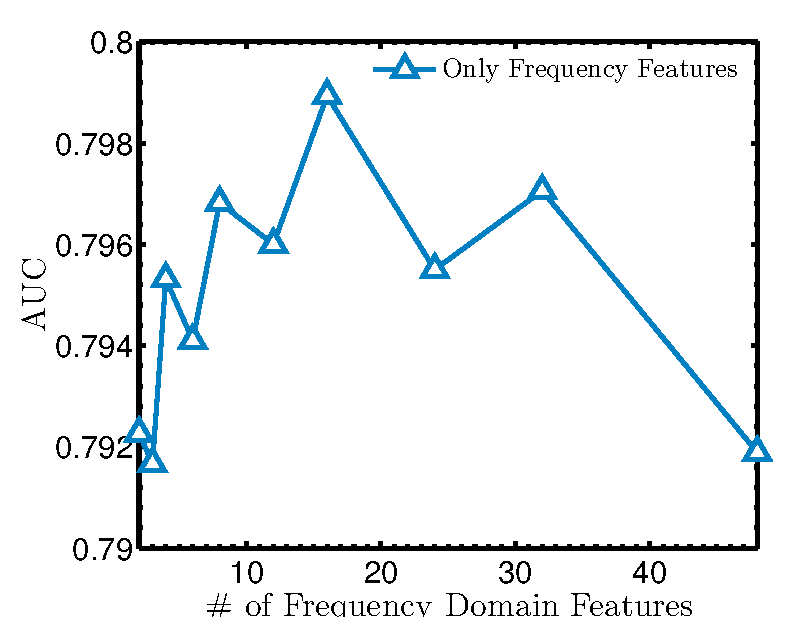
\includegraphics[height=40mm]{fig/fftauc.eps}
    \caption{AUC vs granularity of features in frequencey domain. Only frequency domain features are used with a logistic classifier. }
    \label{fig:FFTAUC}
    \end{minipage}
    \begin{minipage}[t]{0.02\textwidth}~
    \end{minipage}
    \begin{minipage}[t]{0.47\textwidth}
    \centering
    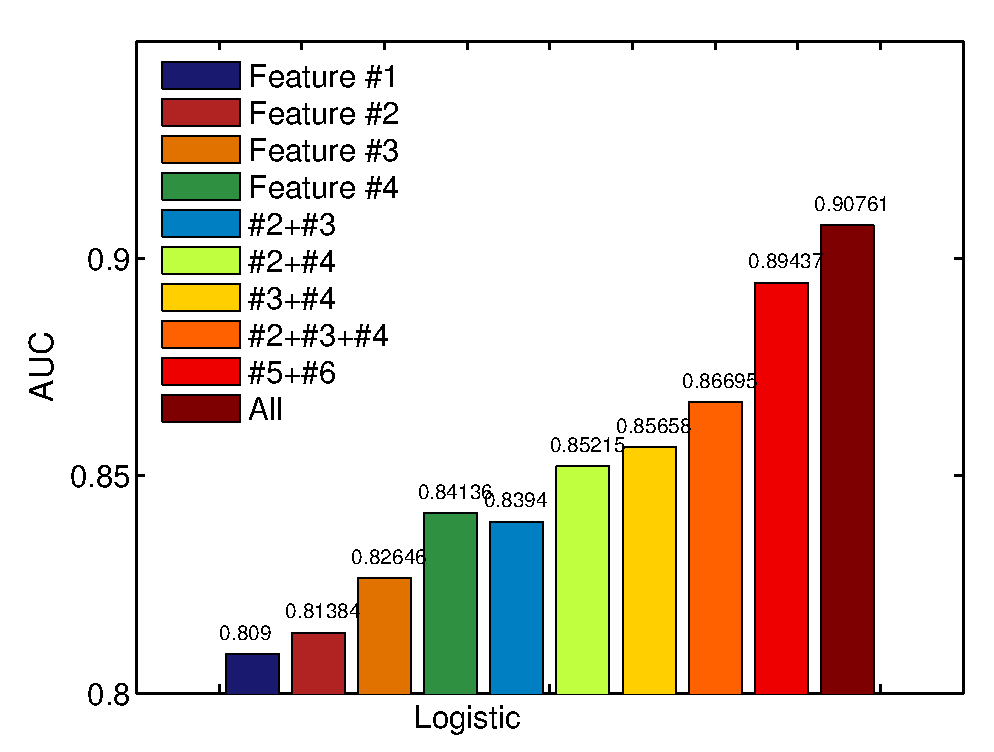
\includegraphics[height=40mm]{fig/feature.eps}\\
    \caption{AUCs vs categories of features used in a logistic classifier. }
    \label{fig:feature}
    \end{minipage}
    \begin{minipage}[t]{0.02\textwidth}~
    \end{minipage}%   
 \end{figure}

Figure \ref{fig:FFTAUC} shows the results. We only applied frequency domain features on our tuned logistic classifier. The results indicates that feature vector within range of 16 to 32 features in frequency domain performance better than smaller or greater ones on average. We can also find that neither smaller or larger number of features performance significantly worse than the optimal ones. This fact means fine-grained feature extraction cannot exploit much more independent features then the coarse-grained ones. The reasons could be 1.Patterns of human movement do not have strong regularity on the frequencies (0 Hz to 2.5 Hz) we investigated, 2. Accelerometer is not sensitive enough to gather that many useful features, 3.the features are there but noise is also strong in that frequency range. If we have device better than cellphone in terms of sensitivity and noise reduction, we could better explain this phenomena.



\subsection{Tuning classifier}
Our preliminary results show that naive K-nearest-neighbour algorithm leads to really poor results which achieve less than 0.6 of AUC. Although there is an important parameter, number of neighbours, for KNN, we simply skip the optimization of KNN for its poor performance and for its consuming computing. 

We use logistic classifier as one of our main options. The only parameter can be tuned in this classifier is $C$ as the weight of logistic regression. It turns out that our features and data is not sensitive to the value of $C$. One possible reason is our feature almost perfectly separates the test data, thus regularity is not very important in this case.

We also tried support vector machine classifier. As its very time-consuming, we use the default value of a SVM with a Gaussian kernel for our classifier.


\subsection{Results}


According to the rules of this competition, classification results were judged on area under the ROC curve. The classifiers we used are k-nearest neighbors, SVM with Gaussian kernel (using LIBSVM) and $L_2$-regularized logistic regression (using LIBLINEAR). The results along with the competition baseline provided by Kaggle (kNN, with the mean of all accelerometer readings as the feature vector for each device in the training set, and the the mean of all readings as the feature vector for each sequence in the testing test), is shown in Table~\ref{tbl:test_result}. For k-nearest neighbors (k-NN-FFT in the table), only the frequency domain features were used, with $k=40$. For SVM with Gaussian kernel, $C=1, \gamma=1$ was used in LIBSVM. For logistic regression (LR-3 in the table), $C=2$ was used in LIBLINEAR.


\begin{table}[!ht]
\caption{Testing results of four methods}
\label{tbl:test_result}
	\begin{center}
		\begin{tabular}{ c | c  c  c  c }
			\hline
			 Methods & k-NN-Mean (baseline) & k-NN-FFT & SVM & LR-3 \\
			 \hline
			 AUC & 0.50277 & 0.58590 & 0.85112 & \textbf{0.90761} \\
			 \hline
		\end{tabular}
	\end{center}
\end{table}

The best results from our approach ranks top 8\% out of 634 teams on Kaggle. Although, the top teams reach over 0.99 of AUC for this competition, the tricky features mentioned in previous section boost the accuracy a lot. According to the online discussion, simply using tricky features to distinguish and identify sensors could achieve the idea results. Although the competition became a game of cheating as it suffers from  "leaks", as quoted from one of the best teams, we, who do not take effort to leverage leaks, show that the reasonable features, which are obtainable in real world, also leads to promising results.

\section{Privacy Control}
In this section we look beyond the competition for a more meaningful and emergent topic, privacy. Results of our approach and others show that using acceleration information, the identity of a person could be easily leaked to others via the mobile devices surrounding us. Before anyone come up with evil ideas based on it, we are urgent to know how much data we can give out before our identities are compromised and in what form the data we provide is safer than other form.

Besides identity, exploiting the raw traces of acceleration make a person even more vulnerable as it could be used for localization with our without the help of GPS. We first investigate how the features impact the accuracy of identification. We assume than distributions like histograms is safer than the frequency domain features. The reason is the data after FFT is still invertible while it is much harder to recovery the time domain trace from histograms. 

The results are shown in figure\ref{fig:feature} and figure\ref{fig:feature_svm}. We use various of combinations of features for the evaluation. The number of features are consistent with the sequence in section\ref{feautures}. Feature \#1 is the frequency domain feature.  Feature \#4 has the best solo-feature classifier. We can achieve over 0.85 for combining features 2, 3 and 4 in a logistic classifier. For the SVM classifier, as it is too time-consuming, we only tried limited combinations and for the full-featured one we only applied 10\% of data on it. These results indicates that 1.using safe features achieves reasonable accuracy for permitted identification without the risk for exploiting more privacy, 2.even exploiting the difference of acceleration or distribution of it still has the risk of make one's identification out of control.

Then we study how the quantity of data impacts the AUC. We vary the size of training data by changing the percentage of data we use. The result is shown in figure\ref{fig:percentage}. The figure shows that when we have a larger training dataset, the AUC, as well as accuracy, increases. The value of AUC increases rapidly within the range between 0.1\% to 10\%. AUC still increases but slows down when a larger dataset is applied. When only 0.1\% of the whole dataset is used, the AUC value is only above 0.7 compared to the baseline of AUC, 0.5. This result indicates that limiting the amount of acceleration data exploited can significantly reduce the accuracy of identification and hence protect the privacy. Meanwhile, we can also find out that the dataset Kaggle provided is more than sufficient.


\section{Conclusion and Future Work}


\begin{figure}
    \hspace{-0.5cm}
    \begin{minipage}[t]{0.02\textwidth}~
    \end{minipage}
    \begin{minipage}[t]{0.47\textwidth}
    \centering
    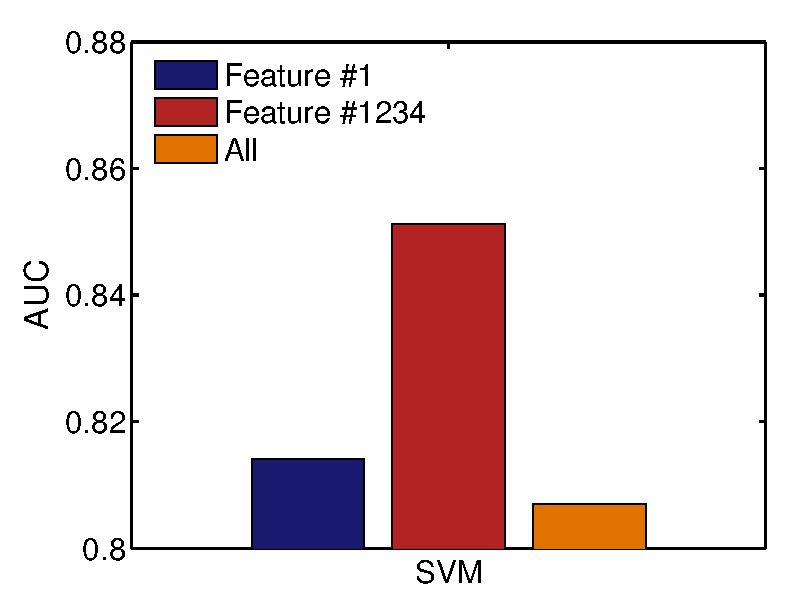
\includegraphics[height=40mm]{fig/feature_svm.eps}
    \caption{AUCs vs categories of features used in a SVM classifier. We only use 10 \% of the whole data for all-feature AUC as it is too time-consuming.}
    \label{fig:feature_svm}
    \end{minipage}
    \begin{minipage}[t]{0.02\textwidth}~
    \end{minipage}
    \begin{minipage}[t]{0.47\textwidth}
    \centering
    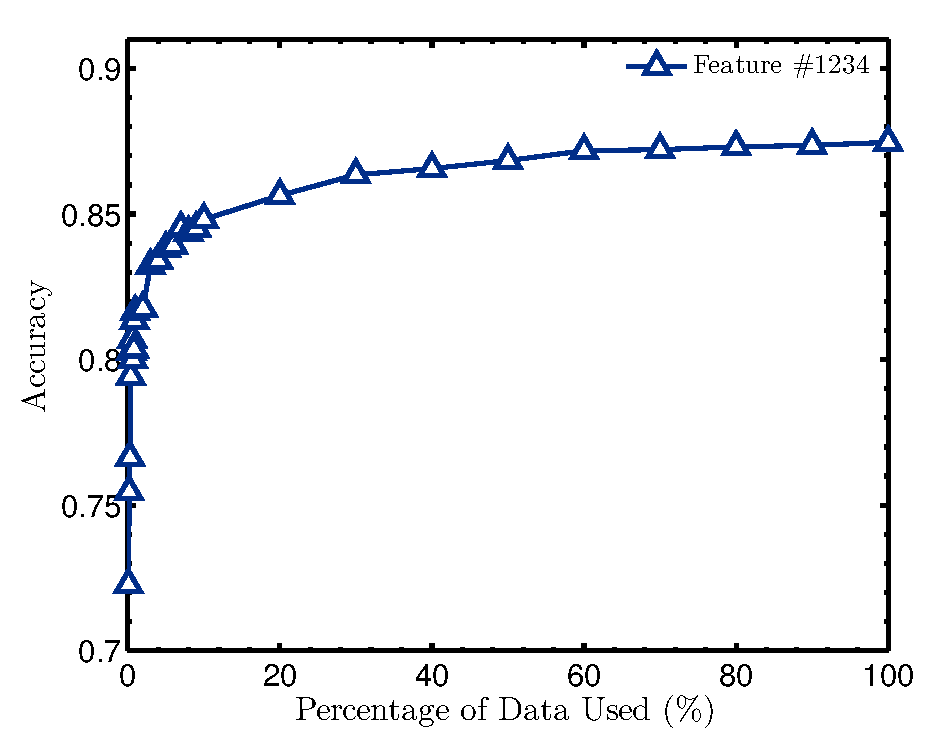
\includegraphics[height=40mm]{fig/percentage.eps}\\
    \caption{AUCs vs percentage of data used in a logistic classifier. }
    \label{fig:percentage}
    \end{minipage}
    \begin{minipage}[t]{0.02\textwidth}~
    \end{minipage}%   
 \end{figure}

We have learned a few things from this project besides a better understanding of machine learning itself as our classifier identifies users well. First, the assumption that human beings have patterns of movement is true. Second, both time domain and frequency domain features help this technique. Third, we have the preliminary knowledge of how to control the leakage of acceleration data to protect our privacy against such technique. By limiting both type and quantity of acceleration data, different goals for protection can be achieved. Furthermore, we can now forecast that applications such as anti-theft, health monitoring and emergency detection that adopt this novel identification technique will be available in the near future.

We could have better results and studies if we get more time in this project. First, the SVM classifier could be tuned more. Second, as we have known the dataset is more than sufficient, we can boost the slow classification program by balancing the accuracy and running time. If we have a device more sensitive than cellphone, we could further studied the patterns of movement and their effectiveness. At last, we are hoping to build a software framework or library for such technique so that it could be more available for practical usage 


\bibliographystyle{IEEEtranS}
\bibliography{references}



\end{document}
